\section{Difference Maps}

The fact that 2D crystals show a higher degree of flexibility can be seen as a disadvantage or as an advantage. On the one hand it limits the resolution on the other hand it makes it easier/possible to investigate conformational changes and thereby provide insight into dynamics of the target protein. For this purpose, one can grow 2D crystals at different conditions, or induce conformational changes \textit{in situ} by incubating the crystals at different conditions during sample preparation. Two different dataset are collected and merged separately. Please make sure that both maps show the same phase origin. Finally, by subtracting the phases and amplitudes of the final maps one can check for significant differences. \\

The difference map is calculated in {\twodx}\texttt{\_merge}. You find the script  \textit{Difference Map}\index{Difference Map} in the Custom Script panel. You can open {\twodx}\texttt{\_merge} in an existing directory or create a new one. In the Parameter panel you have to specify the path for the two merged  \textit{2D.mtz} files (3), enter the right unit cell dimensions (1) and the resolution cutoff (2) you want to apply for the difference map (see \autoref{fig:diffmap1}). Furthermore you can change the contour mode (4), contour range (5) and contour level (6) of you created maps. The script generates a map for both datasets and calculates the difference map with or without superimposed to the first map (7).  

\begin{figure}[H]
		\centering
		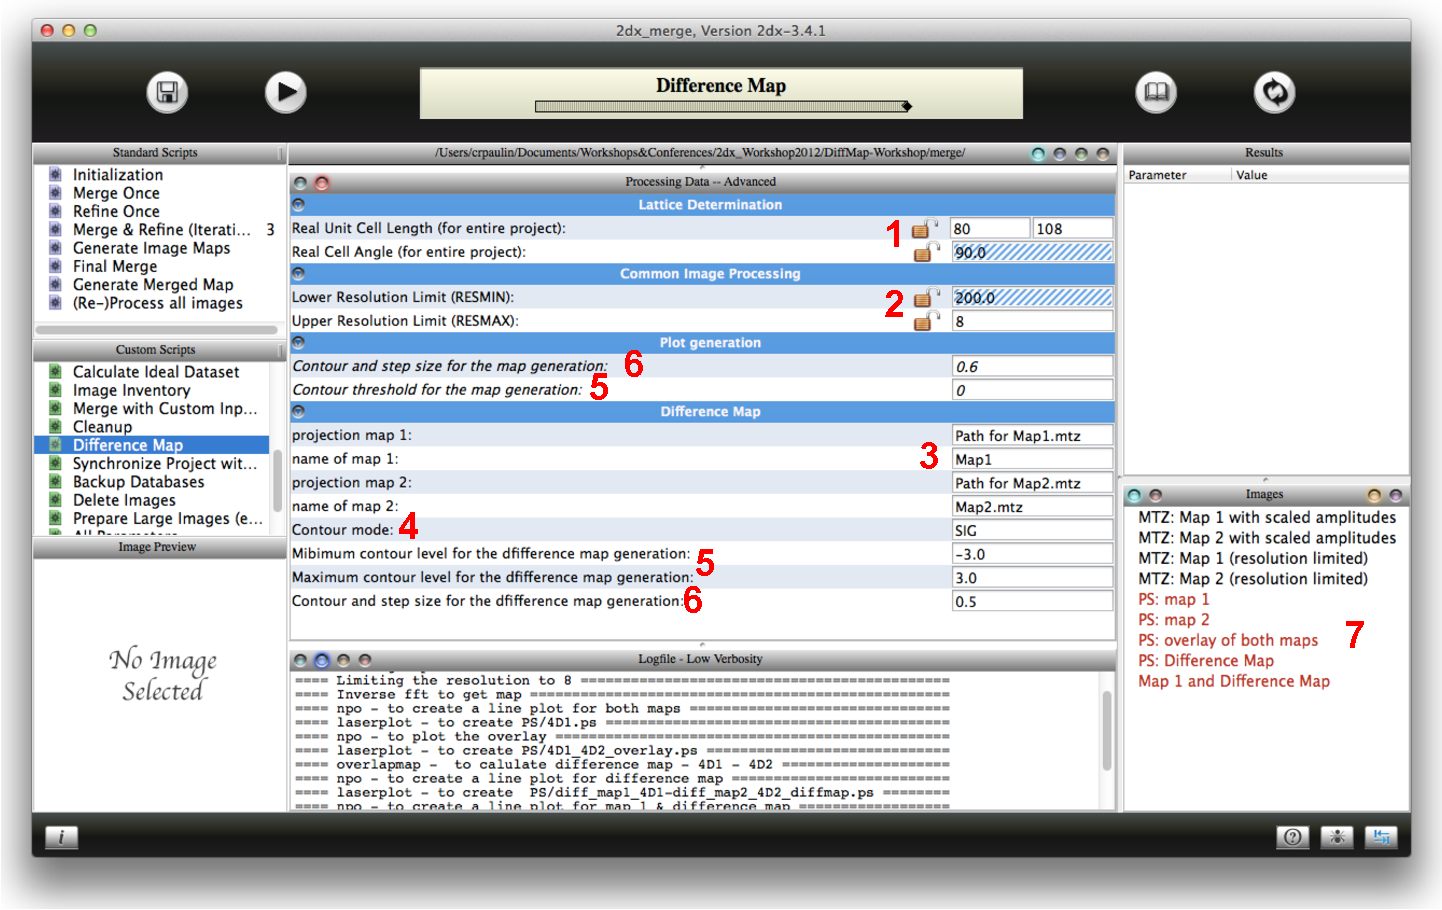
\includegraphics[width=\textwidth]{diffmap1.pdf}
		\caption{GUI for the calculation of a difference map.}.
		\label{fig:diffmap1}
	\end{figure}
	
A way to define the contour level for a "significant difference" is to divide the images of one dataset into two and process them separately. A difference map between these two datasets should give you a range for the noise level.  Hence, you could change the contour level to two levels by changing the \textit{step size for map generation} and define this as your noise level. If you now use this step size for the difference map of interest you can assume that everything above two contour levels is a significant difference. 